



\documentclass[first=dgreen,second=purple,logo=yellowexc]{aaltoslides}
%\documentclass{aaltoslides} % DEFAULT
%\documentclass[first=purple,second=lgreen,logo=redque,normaltitle,nofoot]{aaltoslides} % SOME OPTION EXAMPLES





% input encode
\usepackage[utf8]{inputenc}


%\usepackage[T1]{fontenc}
%\usepackage{lastpage}
%\usepackage{multirow}
%\usepackage{colortbl}
%\usepackage{comment}
%\usepackage{bm}
%\usepackage{natbib}


% Lipsum package generates bullshit
%\usepackage{lipsum}

% Set the document languages
%\usepackage[finnish,swedish,english]{babel}

% nomenclature
%\usepackage[intoc]{nomencl}

% math
\usepackage{amsmath}

% bibliograph
%\usepackage{natbib}

% For algorithms
\usepackage{algorithm}
\usepackage{algorithmic}

% math font
\usepackage{amsfonts}

% theory
%\usepackage{amsthm}

% double bracket
\usepackage{stmaryrd}

% special math symbol
\usepackage{amssymb}

% use enumerate environment
%\usepackage{enumitem}

% use \url \hyperref, make reference clickable
\usepackage{hyperref}

% use lastpage to inde
\usepackage{lastpage}



%-------------------
%
% set
%
%-------------------
\newcommand{\Acal}{\mathcal{A}}
\newcommand{\Bcal}{\mathcal{B}}
\newcommand{\Ccal}{\mathcal{C}}
\newcommand{\Dcal}{\mathcal{D}}
\newcommand{\Ecal}{\mathcal{E}}
\newcommand{\Fcal}{\mathcal{F}}
\newcommand{\Gcal}{\mathcal{G}}
\newcommand{\Hcal}{\mathcal{H}}
\newcommand{\Ical}{\mathcal{I}}
\newcommand{\Jcal}{\mathcal{J}}
\newcommand{\Kcal}{\mathcal{K}}
\newcommand{\Lcal}{\mathcal{L}}
\newcommand{\Mcal}{\mathcal{M}}
\newcommand{\Ncal}{\mathcal{N}}
\newcommand{\Ocal}{\mathcal{O}}
\newcommand{\Pcal}{\mathcal{P}}
\newcommand{\Qcal}{\mathcal{Q}}
\newcommand{\Rcal}{\mathcal{R}}
\newcommand{\Scal}{\mathcal{S}}
\newcommand{\Tcal}{\mathcal{T}}
\newcommand{\Ucal}{\mathcal{U}}
\newcommand{\Vcal}{\mathcal{V}}
\newcommand{\Wcal}{\mathcal{W}}
\newcommand{\Xcal}{\mathcal{X}}
\newcommand{\Ycal}{\mathcal{Y}}
\newcommand{\Zcal}{\mathcal{Z}}

\newcommand{\RR}{\mathbb{R}}
\newcommand{\ZZ}{\mathbb{Z}}

%-------------------
%
% vector
%
%-------------------
\newcommand{\va}{\mathbf {a}}
\newcommand{\vb}{\mathbf {b}}
\newcommand{\vc}{\mathbf {c}}
\newcommand{\vd}{\mathbf {d}}
\newcommand{\ve}{\mathbf {e}}
\newcommand{\vf}{\mathbf {f}}
\newcommand{\vg}{\mathbf {g}}
\newcommand{\vh}{\mathbf {h}}
\newcommand{\vi}{\mathbf {i}}
\newcommand{\vj}{\mathbf {j}}
\newcommand{\vk}{\mathbf {k}}
\newcommand{\vl}{\mathbf {l}}
\newcommand{\vm}{\mathbf {m}}
\newcommand{\vn}{\mathbf {n}}
\newcommand{\vo}{\mathbf {o}}
\newcommand{\vp}{\mathbf {p}}
\newcommand{\vq}{\mathbf {q}}
\newcommand{\vr}{\mathbf {r}}
\newcommand{\vs}{\mathbf {s}}
\newcommand{\vt}{\mathbf {t}}
\newcommand{\vu}{\mathbf {u}}
\newcommand{\vv}{\mathbf {v}}
\newcommand{\vw}{\mathbf {w}}
\newcommand{\vx}{\mathbf {x}}
\newcommand{\vy}{\mathbf {y}}
\newcommand{\vz}{\mathbf {z}}
\newcommand{\vmu}{\mathbf {\mu}}
\newcommand{\valpha}{\mathbf {\alpha}}
\newcommand{\vlambda}{\mathbf {\lambda}}
\newcommand{\vAlpha}{\mathbf {\Alpha}}
\newcommand{\vbeta}{\mathbf {\beta}}
\newcommand{\vBeta}{\mathbf {\Beta}}
\newcommand{\vgamma}{\mathbf {\gamma}}
\newcommand{\vGamma}{\mathbf {\Gamma}}
\newcommand{\vdelta}{\mathbf {\dalta}}
\newcommand{\vDelta}{\mathbf {\Dalta}}
\newcommand{\vone}{\mathbf {1}}
\newcommand{\vzero}{\mathbf {0}}
\newcommand{\vell}{\mathbf {\ell}}
\newcommand{\vxi}{\mathbf{\xi}}
\newcommand{\vphi}{\mathbf{\phi}}
\newcommand{\vPhi}{\mathbf{\Phi}}

%-------------------
%
% math operation
%
%-------------------
\newcommand{\argmax}{\textbf{argmax}}
\newcommand{\argmin}{\textbf{argmin}}
\newcommand{\sign}{\textbf{sign}}
\newcommand{\maximize}{\textbf{max}}
\newcommand{\minimize}{\textbf{min}}
\newcommand{\argkmax}{\textbf{argkmax}}
\newcommand{\argkmin}{\textbf{argkmin}}
\newcommand{\kmaximize}{\textbf{kmax}}
\newcommand{\kminimize}{\textbf{kmin}}
\newcommand{\st}{\textbf{s.t.}}
\newcommand{\set}[1]{\{ #1 \}}
%\newcommand{\ind}[1]{{\llbracket #1 \rrbracket}}
\newcommand{\ind}[1]{\mathbf{1}_{\{#1\}}}
\newcommand{\norm}[1]{\left|\left| #1 \right|\right|}
\newcommand{\ip}[2]{\langle #1, #2 \rangle}
\newcommand{\var}{\textbf{Var}}
\newcommand{\E}{\textbf{E}}
\newcommand{\exponential}[1]{e^{ #1 }}


\newcommand{\Gva}{G_{\va}}
%-------------------
%
% writings
%
%-------------------
\newcommand{\eqdef}{\overset{{\rm \mbox{\tiny def}}}{=}}
\newcommand{\sbf}[1]{\boldsymbol{#1}}
\newcommand{\mbf}[1]{\mathbf{#1}} 
\newcommand{\etal}{{\em et al.}}

\newcommand{\svmstruct}{{\sc ssvm}}
\newcommand{\mmmn}{{\sc m$^3$n}}
\newcommand{\svm}{{\sc svm}}
\newcommand{\mmcrf}{{\sc mmcrf}}
\newcommand{\smo}{{\sc smo}}
\newcommand{\crf}{{\sc crf}}
\newcommand{\nphard}{$\Ncal\Pcal$-hard}
\newcommand{\nphardness}{$\Ncal\Pcal$-hardness}
\newcommand{\iis}{{\sc iis}}
\newcommand{\memm}{{\sc memm}}
\newcommand{\lr}{{\sc lr}}
\newcommand{\svmlight}{{\sc svmlight}}
\newcommand{\libsvm}{{\sc libsvm}}
\newcommand{\svmcascade}{{\sc svmcascade}}
\newcommand{\adaboost}{{\sc adaboost}}
\newcommand{\adaboostmh}{{\sc adaboost.mh}}
\newcommand{\bagging}{{\sc bagging}}
\newcommand{\vrtree}{{\sc vr-tree}}
\newcommand{\deepboosting}{{\sc deepboosting}}
\newcommand{\loo}{{\sc loo}}
\newcommand{\mtl}{{\sc mtl}}
\newcommand{\sdp}{{\sc sdp}}
\newcommand{\iqp}{{\sc iqp}}
\newcommand{\qp}{{\sc qp}}
\newcommand{\daggraph}{{\sc dag}}
\newcommand{\lp}{{\sc lp}}

\newcommand{\hatf}{{\hat{f}}}
\newcommand{\p}{\sc p}
\newcommand{\n}{\sc n}
\newcommand{\pp}{\sc pp}
\newcommand{\pn}{\sc pn}
\newcommand{\nn}{\sc nn}
\newcommand{\maxcut}{{\sc max-cut}}
\newcommand{\greedy}{{\sc greedy}}
\newcommand{\kernelcascade}{{\sc kernel cascade}}
\newcommand{\netrate}{{\sc netrate}}
\newcommand{\netinf}{{\sc netinf}}
\newcommand{\spin}{{\sc spin}}
\newcommand{\vI}{\mathbf{I}}
\newcommand{\tp}{^{\intercal}}
\newcommand{\mve}{{\sc mve}}
\newcommand{\amm}{{\sc amm}}
\newcommand{\mam}{{\sc mam}}
\newcommand{\rta}{{\sc rta}}
\newcommand{\lasso}{{\sc lasso}}
\newcommand{\mle}{{\sc mle}}
\newcommand{\map}{{\sc map}}
\newcommand{\rbf}{{\sc rbf}}
\newcommand{\mlknn}{{\sc ml-knn}}
\newcommand{\knn}{{\sc knn}}
\newcommand{\iblr}{{\sc iblr}}
\newcommand{\cc}{{\sc cc}}
\newcommand{\pcc}{{\sc pcc}}
\newcommand{\ecc}{{\sc ecc}}
\newcommand{\br}{{\sc br}}
\newcommand{\corrlog}{{\sc corrlog}}
\newcommand{\ilgs}{{\sc ilgs}}
\newcommand{\ilrs}{{\sc ilrs}}
\newcommand{\cpp}{{\sc c}}
\newcommand{\matlab}{{\sc matlab}}
\newcommand{\openmp}{{\sc openmp}}
\newcommand{\python}{{\sc python}}
\newcommand{\cvx}{{\sc cvx}}
\newcommand{\lda}{{\sc lda}}
\newcommand{\kkt}{{\sc k.k.t}}
\newcommand{\lbp}{{\sc lbp}}
\newcommand{\anova}{{\sc anova}}

\renewcommand{\algorithmicrequire}{\textbf{Input:}}
\renewcommand{\algorithmicensure}{\textbf{Output:}}



\newcommand{\Upsilonb}{\pmb \Upsilon}
\newcommand{\phib}{\pmb \phi}
\newcommand{\psib}{\pmb \psi}
\newcommand{\varphib}{\pmb \varphi}
\newcommand{\phibh}{\hat\phib}
\newcommand{\psibh}{\hat \psib}
\newcommand{\vYcal}{\pmb \Ycal}
\newcommand{\vXcal}{\pmb \Xcal}
\newcommand{\vFcal}{\pmb \Fcal}
%-------------------
%
% others
%
%-------------------




%\newtheorem{definition}{Definition}
%\newtheorem{theory}{Theory}
%\newtheorem{lemma}{Lemma}

















\title{Max-Margin Learning with A Random Sample of Spanning Trees}
\author{Hongyu Su}



\institute[ICS]{
Helsinki Institute for Information Technology HIIT\\
Department of Computer Science\\
Aalto University
}

\aaltofootertext{Random Spanning Tree Approximation}{\today}{\arabic{page}/\pageref{LastPage}\ }


\date{ \today} %\date{Version 1.0, \today}

\iffalse
\AtBeginSection[]
{
  \begin{frame}<beamer>{Outline}
    \tableofcontents[currentsection,subsection]
  \end{frame}
}
\fi




%--------------------------------
%
% document
%
%--------------------------------

\begin{document}

\aaltotitleframe



%
\begin{frame}{Multilabel classification}
	\begin{itemize}
		\item Multilabel classification is an important research field in machine learning.
		\begin{itemize}
			\item For example, a document can be classified as ``science'', ``genomics'', and ``drug discovery''.
			\item Each input variable $\vx\in\vXcal$ is associated with multiple output variables $\vy\in\vYcal,\vYcal=\Ycal_1\times\cdots\times\Ycal_l,\Ycal_i=\{+1,-1\}$.
			\item The goal is to find a mapping function that predicts the best values of an output given an input $f\in\Hcal:\vXcal\rightarrow\vYcal$.
		\end{itemize}
		\item The central problems of multilabel classification:
		\begin{itemize}
			\item The size of the output space $\vYcal$ is exponential in the number of microlabels.
			\item The dependency of microlabels needs to be exploited to improve the prediction performance.
		\end{itemize}
	\end{itemize}
\end{frame}



%
\begin{frame}{Structured output learning}
	\begin{itemize}
		\item There is an \textit{output graph} connecting multiple labels.
		\begin{itemize}
			\item A set of nodes represents multiple labels.
			\item A set of edges represents the correlation between labels.
		\end{itemize}
		\item Hierarchical classification:
		\begin{itemize}
			\item The output graph is a rooted tree or a directed graph defining different levels of granularities.
			\item For example, \svmstruct, ...
		\end{itemize}
		\item Graph labeling:
		\begin{itemize}
			\item The output graph often takes a general form (e.g., a tree, a chain).
			\item For example, \mmmn, \crf, \mmcrf, ...
		\end{itemize}
		\item The output graph is assumed to be known \textit{apriori}.
	\end{itemize}
\end{frame}



%
\begin{frame}{Research question}
	\begin{itemize}
		\item The output graph is hidden in many applications.
		\begin{itemize}
			\item For example, a surveillance photo can be tagged with ``building'', ``road'', ``pedestrian'', and ``vehicle''.
		\end{itemize}
		\item We study the problem in structured output learning when the output graph is not observed.
		\item In particular:
		\begin{itemize}
			\item Assume the dependency can be expressed by a complete set of pairwise correlations.
			\item Build a structured output learning model with a complete graph as the output graph.
			\item Solve the optimization problem and the inference problem (\nphard).
		\end{itemize}
	\end{itemize}
\end{frame}



%
\begin{frame}{In this presentation}
	\begin{itemize}
		\item A structured prediction model which performs max-margin learning on a random sample of spanning tree.
		\item Two ways to combine the set of random spanning trees.
		\begin{itemize}
			\item conical combination
			\item convex combination
		\end{itemize}
		\item The corresponding optimization problem.
	\end{itemize}
\end{frame}



%
\begin{frame}[allowframebreaks]{Model}
	\begin{itemize}
		\item Training examples comes in pair $S=\{(\vx_i,\vy_i)\}_{i=1}^{m}\in\vXcal\times\vYcal$.
		\item A complete graph $G=(E,V)$ is used as the output graph.
		\item $\Gamma_G(\vy_i)$ is the output feature map of $\vy_i$ on $G$
		\begin{align*}
			\Gamma_G(\vy_i) &= \{\Gamma_e(\vy_{i,e})\}_{e\in G},\\
			 \Gamma_e(\vy_{i,e}) &= [\vone_{\vy_{i,e}==00},\vone_{\vy_{i,e}==01},\vone_{\vy_{i,e}==10},\vone_{\vy_{i,e}==11}]
		\end{align*}
		\item A joint feature map of $(\vx_i,\vy_i)$
		\begin{align*}
			\phi_G(\vx_i,\vy_i) = \varphi(\vx_i)\otimes\Gamma_G(\vy_i) = \{\phi_e(x_i,\vy_{i,e})\}_{e\in G}.
		\end{align*}
		\item A compatibility score is defined as
		\begin{align*}
			F(\vx,\vy;\vw_G) = \ip{\vw_G}{\phi_G(\vx,\vy)}=\sum_{e\in G}\ip{\vw_{G,e}}{\phi_e(\vx,\vy_{e})}
		\end{align*} 
		\item $\vw$ ensures an input $\vx_i$ with a correct multilabel $\vy_i$ achieves a higher score than with any incorrect multilabel $\vy\in\Ycal$.
		\item The predicted output $\vy(\vx)$ for a given input $\vx$ is computed by
		\begin{align*}
			\vy(\vx) = \underset{\vy\in\vYcal}{\argmax}\,F(\vx,\vy;\vw_G) = \underset{\vy\in\vYcal}{\argmax}\,\ip{\vw_G}{\phi_G(\vx,\vy)},
		\end{align*}
		which is called \textit{inference problem}.
		\item The {inference problem} is \nphard\ for most joint feature maps on the complete graph.
	\end{itemize}
\end{frame}



%
\begin{frame}{How to learn $\vw$ on a complete graph?}
	\begin{itemize}
		\item The \textit{margin} of an example $\vx_i$ is
		\begin{align*}
			\gamma_G(\vx_i;\vw_G) = F(\vx_i,\vy_i;\vw_G) - \underset{\vy\in\vYcal/\vy_i}{\maximize}\,F(\vx_i,\vy;\vw_G).
		\end{align*}
		\item $\vw$ is solved by \textit{maximum-margin principle} which aims to maximize $\gamma(\vx_i;\vw_G)$ over all training example.
		\item The problems are:
		\begin{itemize}
			\item The \nphardness\ of the inference problem on a complete graph.
			\item A large parameter space: $\Theta(k^2)$
		\end{itemize}
		\item We aim to use a joint feature map that allows the inference problem be solved in polynomial time.
	\end{itemize}
\end{frame}



%
\begin{frame}{Superposition of random trees}
	\begin{itemize}
		\item $U(G)$ is a complete set of spanning tree generate from $G$.
		\item $\vw_{T}=\{\vw_{G,e}\}_{e\in T}$ is the projection of $\vw_G$ on $T$.
		\item $\phi_T(\vx,\vy)=\{\phi_e(\vx,\vy)\}_{e\in T}$ is the projection of $\phi_G(\vx,\vy)$ on $T$.
		\item Rewrite
		\begin{align*}
			F(\vx,\vy,\vw_G) &= \sum_{e\in G}\ip{\vw_{G,e}}{\phi_{G,e}(\vx,\vy_e)} \\
			& = \frac{1}{\ell^{\ell-2}}\sum_{T\in U(G)}\sqrt{\frac{\ell}{2}}\ip{\vw_{T}}{\phi_{T}(\vx,\vy_e)}\\
			& = \esp{T\in U(G)}a_{T}\ip{\hat{\vw}_{T}}{\hat{\phi}_{T}(\vx,\vy_e)},\\
			&\esp{T\in U(G)} a_T^2=1, \quad 	\esp{T\in U(G)} a_T\le1.
		\end{align*}
	\end{itemize}
\end{frame}

%
\begin{frame}{Random Spanning Tree Approximation}
	\begin{itemize}
		\item We proved if a large margin structured output predictor exists, then combining a small sample of random trees will, with a high probability, generate a predictor with good generalization.
		\item $\Tcal=\{T_1,\cdots,T_n\}$ is a set of spanning trees randomly sampled from the complete graph $G$.
		\item The compatibility score can be re-defined based on $\Tcal$ as
		\begin{align*}
			F_{\Tcal}(\vx_i,\vy_i;\vw_{\Tcal}) = \sum_{t=1}^{n}\ip{\vw_{T_t}}{\phi_{T_t}(\vx_i,\vy_i)}.
		\end{align*}
		\item The inference problem of predicting the output $\vy_{\Tcal}(\vx)$ for a given input $\vx$ is 
		\begin{align*}
			\vy_{\Tcal}(\vx) = \underset{\vy\in\vYcal}{\argmax}\,F_{\Tcal}(\vx,\vy;\vw_{\Tcal})=\underset{\vy\in\vYcal}{\argmax}\,\sum_{t=1}^{n}\ip{\vw_{T_t}}{\phi_{T_t}(\vx,\vy)}.
		\end{align*}
	\end{itemize}
\end{frame}


%
\begin{frame}{Optimization Problem}
	\begin{itemize}
		\item The margin of an example $\vx_i$ achieved by $\Tcal$ is
		\begin{align*}
		\gamma_{\Tcal}(\vx_i;\vw_{\Tcal}) = \underset{\vy\in\vYcal/\vy_i}{\minimize}\,[\sum_{t=1}^{n}\ip{\vw_{T_t}}{\phi_{T_t}(\vx_i,\vy_i)}-\sum_{t=1}^{n}\ip{\vw_{T_t}}{\phi_{T_t}(\vx_i,\vy)}].
	\end{align*}
		\item To learn $\{\vw_{T_t}\}_{T_t\in\Tcal}$ we solve the optimization problem
		\begin{align*}
			\underset{\vw_{T_t},\xi_i}{\minimize} & \quad \frac{1}{2}\sum_{t=1}^{n}\norm{\vw_{T_t}}^2 + C\sum_{i=1}^{m}\xi_i\\
			\st & \quad \sum_{t=1}^{n}{ \langle \vw_{T_t}, \phib_{T_t}(\vx_i,\vy_i) \rangle} - \underset{\vy \neq \vy_i}{\maximize\ } \sum_{t=1}^{n}{\langle \vw_{T_t}, \phib_{T_t}(\vx_i,\vy) \rangle } \geq 1 -  \xi_i, \\
			& \quad \xi_i\ge0\, , \forall\ i \in \set{1,\dots,m},
		\end{align*}
	\end{itemize}
\end{frame}



%
\begin{frame}{Inference Problem}
	\begin{itemize}
		\item The inference problem of \rta\ is defined as finding the multilabel $\vy_{\Tcal}(\vx)$ that maximizes the sum of scores over a collection of trees
		\begin{align*}
			\vy_{\Tcal}(\vx) = \underset{\vy\in\vYcal}{\argmax}\,{\color{aaltoblue}F_{\Tcal}(\vx,\vy;\vw_{\Tcal})} = \underset{\vy\in\vYcal}{\argmax}\,\sum_{t=1}^{n}\ip{\vw_{T_t}}{\phi_{T_t}(\vx,\vy)}.
		\end{align*}
		\item The inference problem on each individual spanning tree can be solve efficiently in $\Theta(l)$ by \textit{dynamic programming}
		\begin{align*}
			\vy_{T_t}(\vx) = \underset{\vy\in\vYcal}{\argmax}\,{\color{aaltored}F_{T_t}(\vx,\vy;\vw_{T_t})}= \underset{\vy\in\vYcal}{\argmax}\,\ip{\vw_{T_t}}{\phi_{T_t}(\vx,\vy)}.
		\end{align*}
		\item There is no guarantee that there exists a tree $T_t\in\Tcal$ in which the maximizer of ${\color{aaltored}F_{T_t}}$ is the maximizer of ${\color{aaltoblue}F_{\Tcal}}$.
	\end{itemize}
\end{frame}




%
\begin{frame}[allowframebreaks]{Fast Inference Over a Collection of Trees}
	\begin{itemize}
		\item For each tree $T_t$, instead of computing the best multilabel $\vy_{T_t}$, we compute $K$-best multilabels in $\Theta(Kl)$ time
		\begin{align*}
			\Ycal_{T_t,K} = \{\vy_{T_t,1},\cdots,\vy_{T_t,K}\}.
		\end{align*}
		\item Performing the same computation on all trees gives a candidate list of $n\times K$ multilabels in $\Theta(nKl)$ time
		\begin{align*}
			\Ycal_{\Tcal,K}=\Ycal_{T_1,K}\cup\cdots\Ycal_{T_n,K}.
		\end{align*}
		\item For now, we assume the best scoring multilabel of a collection of trees exists in the list $\Ycal_{\Tcal,K}$. 
		\item Assume 
		\begin{align*}
		\vy_K^*=\underset{\vy\in\Ycal_{\Tcal,K}}{\argmax}\,F_{\Tcal}(\vx,\vy;\vw_{\Tcal}).
		\end{align*} 
		If
		\begin{align*}
			F_{\Tcal}(\vx,\vy_K^*;\vw_{\Tcal})\ge\frac{1}{n}\sum_{t=1}^{n}F_{T_t}(\vx,\vy_{T_t,K},\vw_{T_t})=\theta_{\vx}(K),
		\end{align*}
		then 
		\begin{align*}
			F_{\Tcal}(\vx,\vy_K^*;\vw_{\Tcal}) = \underset{\vy\in\vYcal}{\maximize}\,F_{\Tcal}(\vx,\vy;\vw_{\Tcal}).
		\end{align*}
		\framebreak
		\item For example, $\Tcal=\{T_1,T_2\},\vYcal=\Ycal_1\times\Ycal_2,\Ycal_i=\{+,-\}$
		\begin{table}
			\begin{tabular}{|c|cc|cc|c|} \hline
				\multirow{2}{*}{} & \multicolumn{2}{c|}{$T_1$} & \multicolumn{2}{c|}{$T_2$} & $\theta_{\vx}(K)$\\ \cline{2-5}
				& $\vy_{T_1,K}$ & $F_{T_1}(\vx,\vy_{T_1,K})$ & $\vy_{T_1,K}$ & $F_{T_1}(\vx,\vy_{T_1,K})$ & \\ \hline
				$K=1$ & $+-$ & $5$ & $--$ & $4$ & $9$\\ \hline
				$K=2$ & $++$ & $4$ & $-+$ & $3$ & $7$\\ \hline
				$K=3$ & $-+$ & $3$ & $++$ & $3$ & $6$\\ \hline
				$K=4$ & $--$ & $3$ & $+-$ & $2$ & $5$\\ \hline
			\end{tabular}
		\end{table}
		\item We proved that with a high probability $\vy_{\Tcal}$ will appear in $\Ycal_{\Tcal,K}$.
	\end{itemize}
\end{frame}



%
\begin{frame}{Performance of the Inference Algorithm}
	\begin{itemize}
		\item $10$ datasets, $|\Tcal| = \{5,10,40\}, K=\{2,4,8,16,32,40,60\}$
		\item X-axis is the percentage of examples with exact inference.
		\item Y-axis is the value of $K$ as the percentage of the number of microlabels.
		\item $K=100\%|Y|$ corresponds to a complexity of $\Theta(nl^2)$.
	\end{itemize}
	\begin{figure}
		\begin{center}
			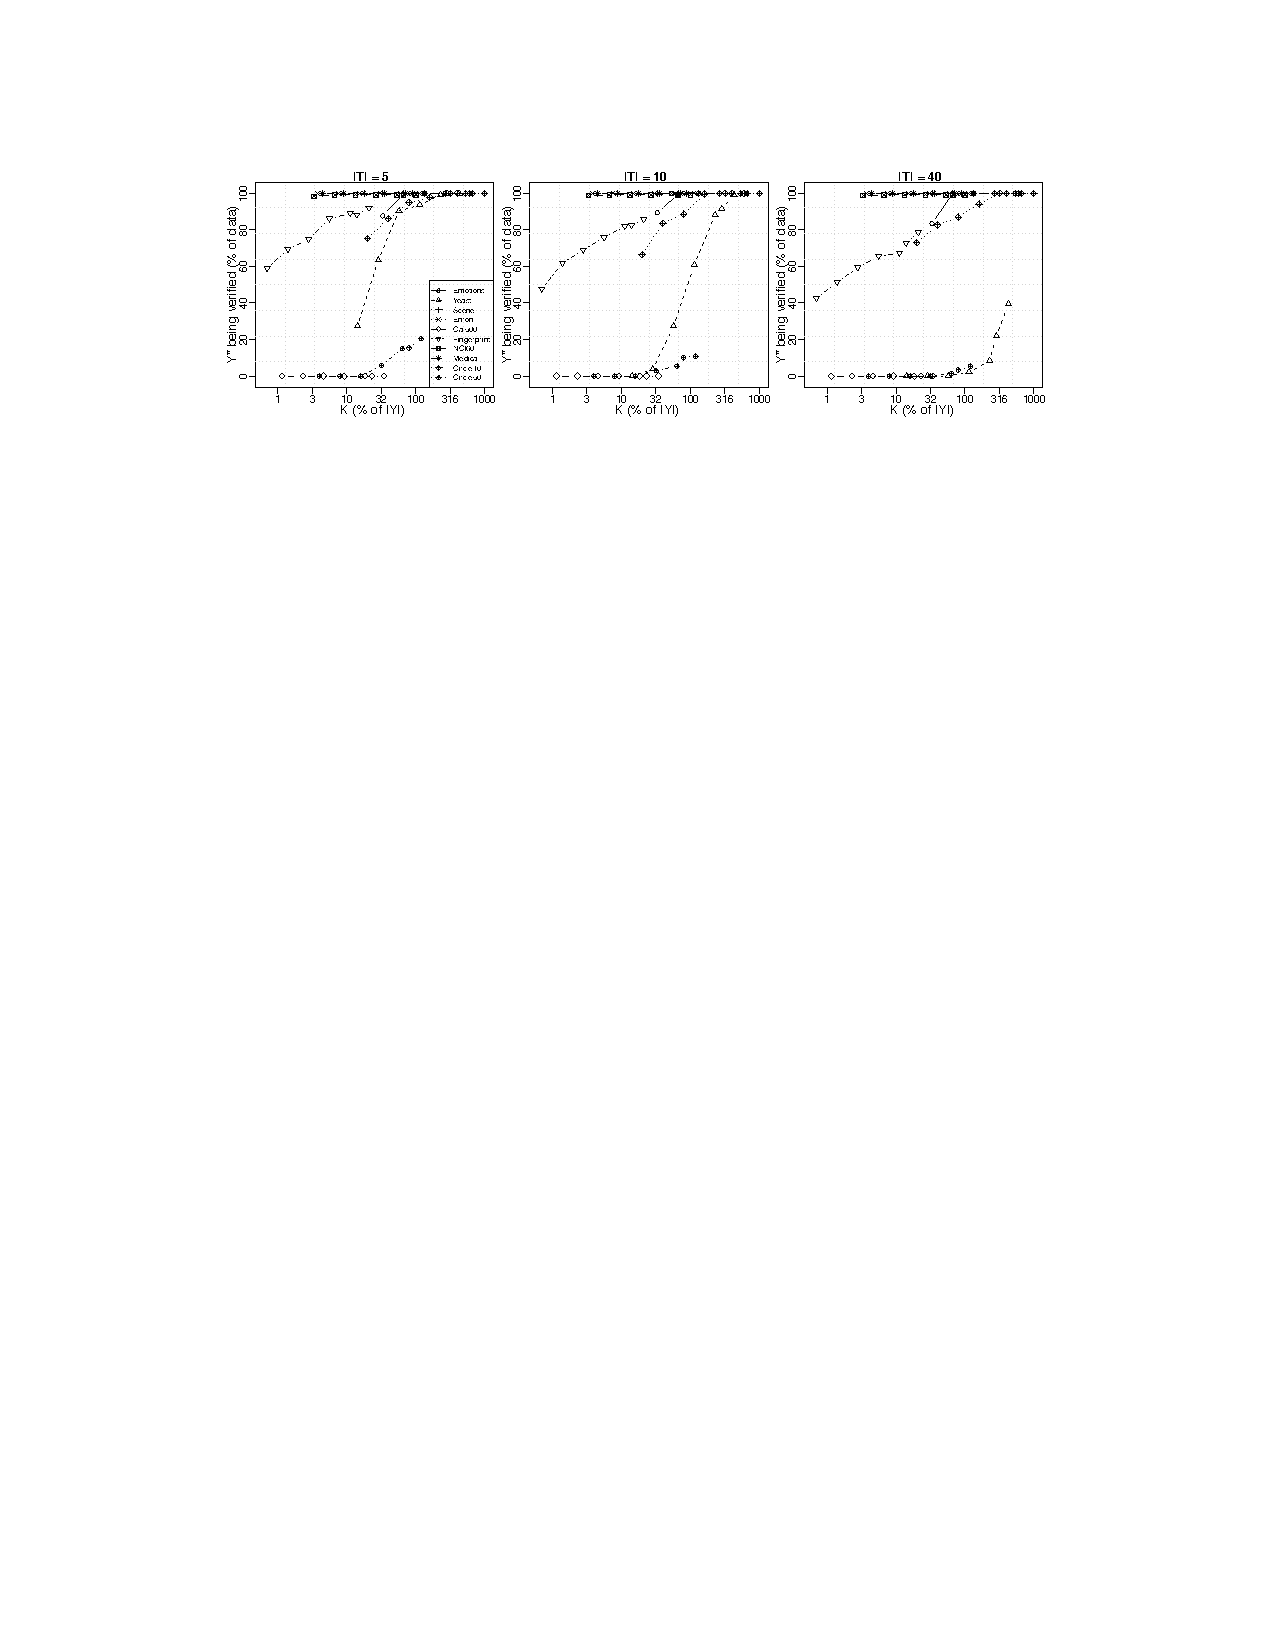
\includegraphics[width=11cm]{./result_plot.pdf}
			%\caption{Percentage of examples with provably optimal $\vy$ being in the $K$-best lists plotted as a function of K, scaled with respect to the number of microlabels in the dataset.}
		\end{center}
	\end{figure}
\end{frame}



%
\begin{frame}{Prediction Performance}
	\begin{figure}
		\begin{center}
			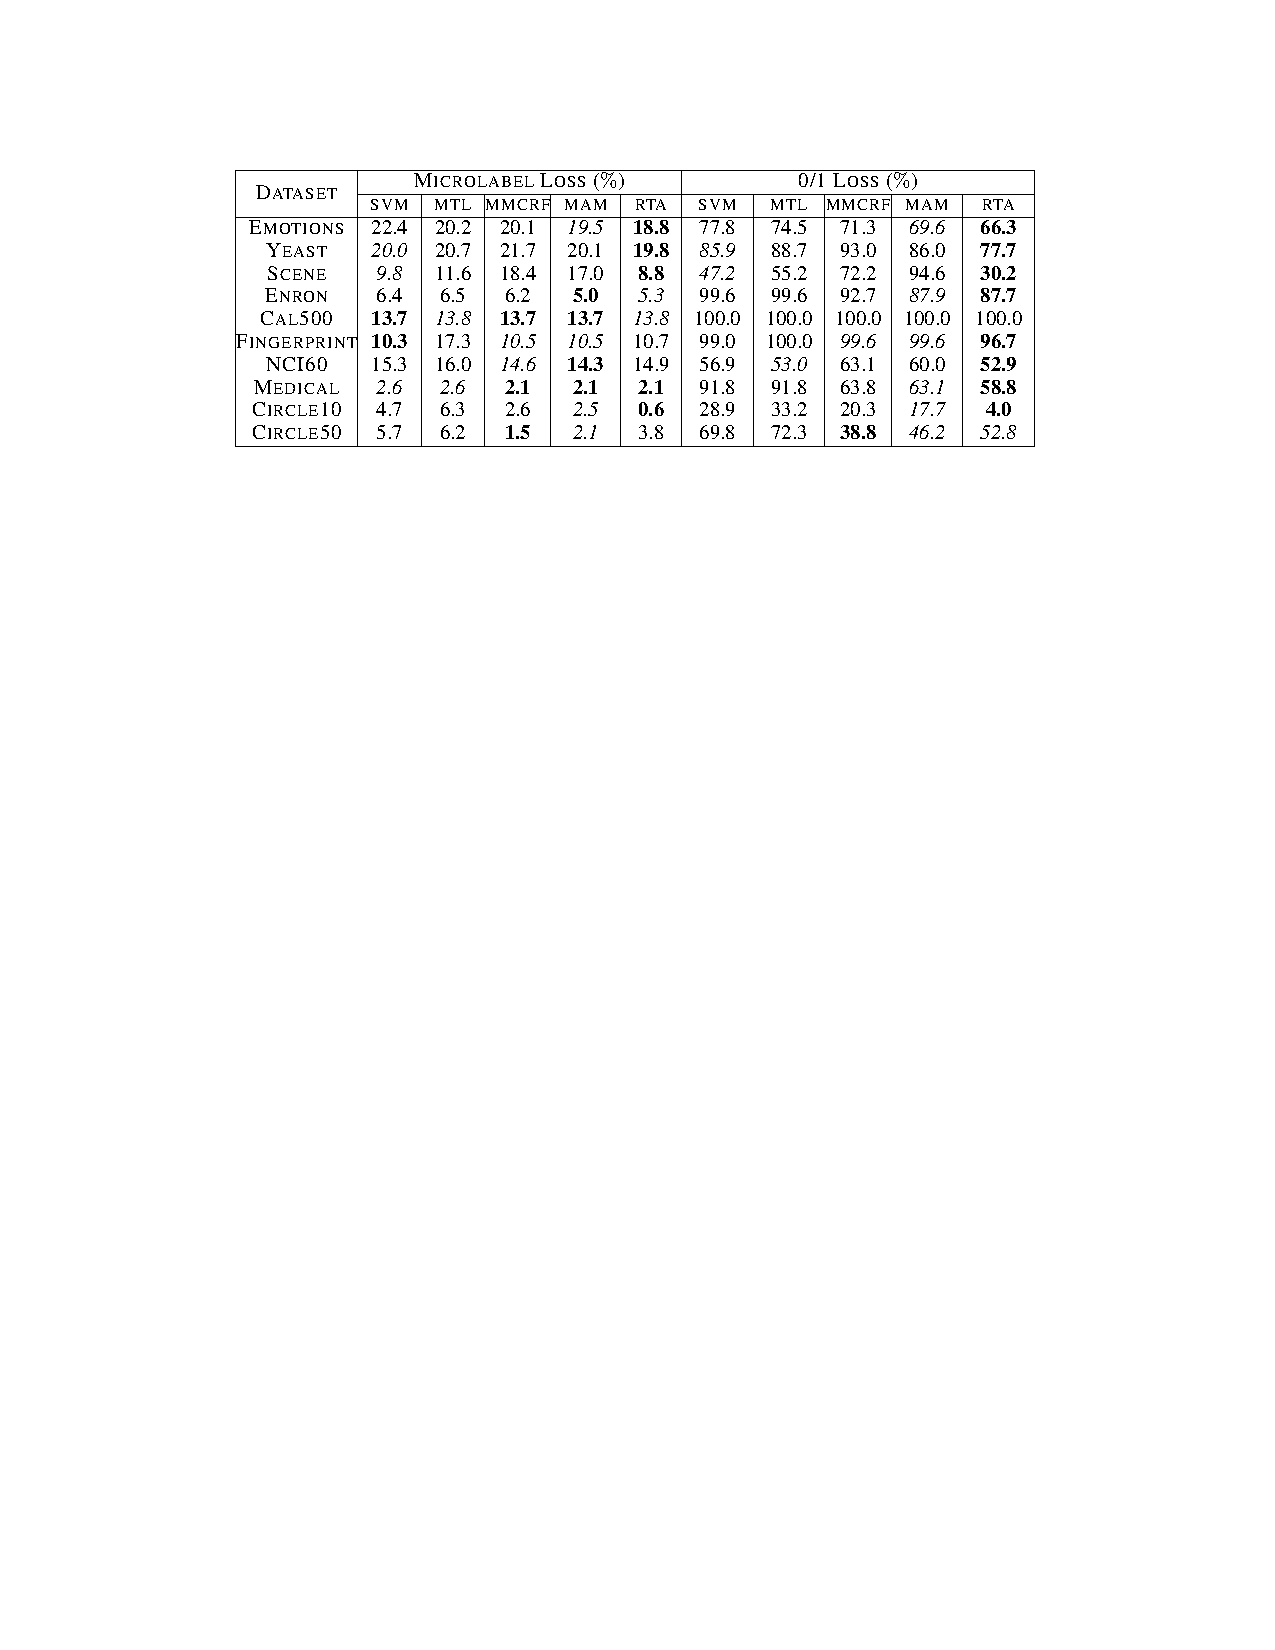
\includegraphics[width=11cm]{./result_table.pdf}
			\caption{Prediction performance of each algorithm in terms of microlabel loss and 0/1 loss. The best performing algorithm is highlighted with boldface, the second best is in italic}
		\end{center}
	\end{figure}
\end{frame}



%
\begin{frame}{Conclusions}
	\begin{itemize}
		\item Theoretical study shows if a large margin structured output learner exists,  then the combination of a random sample of spanning trees will achieve a similar margin with a high probability.
		\item The $K$-best inference algorithm is tractable which is proved theoretically and empirically.
		\item \rta\ is not constrained by the availability of the output graph, it can therefore be applied to a wider range of multilabel classification problem where the output graph is believed to play an important role during learning.
	\end{itemize}
\end{frame}




\iffalse
\begin{frame}[allowframebreaks]{Bibliography}
	%\bibliographystyle{plain}
	\bibliographystyle{apalike}
	\bibliography{example}
\end{frame}
\fi


\end{document}
